\documentclass{cys}

\usepackage[utf8]{inputenc}

%\usepackage[english]{babel}
%\usepackage[spanish,mexico,es-tabla]{babel}
\usepackage[russian,english]{babel}  % If you use other languages, use Babel package.


\usepackage{graphicx}
\usepackage{amsmath,amssymb}
\usepackage{float,epstopdf} % Avoid using plain Latex, use PDFLATEX
\usepackage[dvipsnames]{xcolor}
\usepackage{hyperref}
\graphicspath{{./Figures/}}
\DeclareGraphicsExtensions{.jpeg,.bmp,.png,.jpg,.eps,.pdf}
\usepackage{adjustbox}
\hypersetup{
    colorlinks=true,
    linkcolor=blue,
    filecolor=magenta,      
    urlcolor=cyan,
    pdftitle={Overleaf Example},
    pdfpagemode=FullScreen,
    }

\addto\captionsenglish{%
  \renewcommand{\figurename}{Fig.}%
  \renewcommand{\abstractname}{Abstract.} 
%  \renewcommand{\keywordsname}{Keywords: } 
}

\addto\captionsspanish{%
  \renewcommand{\figurename}{Fig.}%
  \renewcommand{\abstractname}{Resumen.} 
%  \renewcommand{\keywordsname}{Palabras clave: } 
}


\title{Geometrical Deep Learning: A Feasible Methodology For Predicting Age}

\author{Santiago Isaac Flores-Alonso $^1$, Blanca Tovar-Corona$^2$, René Luna-García$^1$}

\affil{ 
$^1$ IPN,CIC, Ciudad de México 07738,   \authorcr   % Do not us full postal address!
México            
\authorcr \authorcr
$^2$ IPN,UPIITA, Ciudad de México 07340, \authorcr
México             
\authorcr  \authorcr
                  
\authorcr  \authorcr
sfloresa2010@alumno.ipn.mx, bltovar@ipn.mx, rlunag@ipn.mx
\authorcr  \authorcr
}


\begin{document}

\maketitle

\renewcommand{\tablename}{Table}

\begin{abstract}
This paper presents...
\end{abstract}

\begin{keywords} 
Aging, cortical features, connectomics, GCN, PSD, , 
\end{keywords} 



\section{Introduction}
\label{sec:introduction}



The human brain undergoes dynamic changes throughout life, with the aging process in adulthood leading to structural and functional changes, contributing to a gradual cognitive decline \cite{yankner2008aging}. Although these age-related changes are not inherently pathological, the likelihood of developing neurodegenerative disorders increases with age \cite{baecker2021machine, nguyen2024brain}. Emerging research suggests that certain neurodegenerative conditions may stem from processes associated with accelerated brain aging \cite{isaev2018accelerated}.

\bigskip In this context, preventive medicine stands to benefit from individualized quantification of atypical aging, as a significant deviation between predicted and chronological age, may indicate pathological aging \cite{lee2023choice}. %Such deviations could be associated with various age-related risk factors, leading to impaired cognitive functions and neuropathologies.

\bigskip
Understanding and identifying biomarkers that define healthy aging is crucial to detect early-stage neurodegeneration and predicting age-related cognitive decline. One promising approach involves leveraging neuroimaging and electrophysiological data to capture the multivariate patterns of age-related brain change and formulate high-dimensional regression boundaries to accurately predict the age of healthy individuals. Machine learning (ML) models, trained on neurotypical subjects, can then be applied to clinical samples, revealing aberrant age-related changes, and offering a population-level tool for assessing brain aging. This approach has been employed in various disorders, such as Alzheimer’s\cite{franke2012longitudinal, gaser2013brainage,gonneaud2020functional, gao2022brain}, traumatic brain injury\cite{cole2015prediction}, schizophrenia \cite{koutsouleris2014accelerated, zhuang1997event}, HIV \cite{kuhn2018augmented, cole2017increased} , epilepsy \cite{pardoe2017structural}, and Down’s syndrome\cite{cole2017brain}. Additionally, predicting brain age has extended beyond neurological disorders, showing positive impacts of meditation\cite{luders2016estimating}, diet \cite{onaolapo2019brain}, increased education and physical exercise \cite{steffener2016differences,vecchio2018neuroprotective}  on brain age. 

\bigskip
The aforementioned studies have focused mainly on estimating brain age based primarily on gray matter morphometry or spectral features from different brain regions of interest (ROIs) independently. Nevertheless, the brain is a network of interleaved neural circuits, 

\bigskip
The aforementioned studies have focused mainly on estimating brain age based primarily on structural features, extracted from magnetic resonance imaging (T1-weighted MRI). Nevertheless, the brain is a network of interleaved neural circuits, where its the majority of functions are supported by coordinated activity between distinct, separated brain regions \cite{sala2015reorganization}, %and only using the morphometric features neglects the underlying topology and functional aspect of the brain, such as information about the neighborhood, the connectivity, or the distribution of power and frequencies among ROIs.

\bigskip
Connectivity measures, which models the brain interleaved neural circuits and represent it as a graph, exhibits important changes during healthy aging and presents specific patterns for different neuropathologies \cite{monti2020interpretable, li2018brain, lin2016predicting}. In the context of incorporating functional, structural, and connectivity information for age prediction, Graph Convolutional Networks (GCN) provide a more suitable architecture since they enable feature embedding in graph nodes, transforming these features while considering the graph topology. To delve into the role of brain topology in age prediction, we implemented a GCN architecture on graphs generated derived from resting-state MEG and structural connectivity measures derived from diffusion MRI, to predict brain age. Each node was annotated by their gray matter morphometry  and spectral features. %Our exploration of age-related brain changes involved utilizing MEG electrophysiological recordings and MRI structural features of each brain region as features for the graph nodes.



\section{Related Work}
\label{sec:relatedWork}

Numerous studies have delved into the intricate dynamics of age-related changes in the human brain, recognizing the crucial role of these alterations in cognitive decline and the onset of neurodegenerative disorders. These investigations underscore the potential of individualized quantification of atypical aging as a means for the early detection of pathological conditions.

\bigskip
In this section, our focus shifts exclusively to works published between 2018 and 2023 that leverage the identical dataset detailed in Section \ref{subsec: Dataset}, either independently or in conjunction with another database. As depicted in Table \ref{table:Table1}, the aforementioned studies predominantly concentrate on estimating brain age based on morphometric or spectral data from different brain regions of interest (ROIs), extracted from structural magnetic resonance imaging (T1-weighted MRI) [cite] and M/EEG data, with the former being the most prevalent and exhibiting the best performance. However, most overlook the underlying topology of the brain, neglecting critical information related to the neighborhood, connectivity, or distribution of power and frequencies among ROIs.

\bigskip
A couple of works have explored topological features using 3D Convolutional Neural Networks (3D CNN), capturing the spatial distribution of gray and white matter in T1-weighted MRI images. Additionally, 2D CNNs have been employed to capture the spatial topology of connectomes \cite{li2022brain}. Nevertheless, CNNs, designed for Euclidean spaces, may yield misleading conclusions when applied to graphs, given their inherent non-Euclidean structure. Furthermore, CNNs cannot incorporate node embeddings in the graph as part of the feature space.

\bigskip
It is essential to note that a variety of feature extraction techniques have been employed, with both linear and nonlinear approaches, demonstrating comparable performance. While these studies validate the effectiveness of their chosen techniques, none has dedicated itself to methodologies that integrate electrophysiological, morphological, and connectomical data into a framework that best aligns with the brain's architecture. In contrast, the present work achieves this integration through the use of Graph Convolutional Networks (GCN).

\begin{table*}[]
\renewcommand{\arraystretch}{1.65}
	\centering
	\caption{Comparative table between works that used the same dataset}
	\rotatebox{90}
{
	\resizebox{1.4\textwidth}{!}{%
\begin{tabular}{llllllll}
\hline
\textbf{Title}                                                                                                                                                                                 & \textbf{Dataset}                                                                                                                               & \textbf{Year} & \textbf{Technique} & \textbf{N}                                                                                                         & \textbf{Features}                                                                                                                                                                                                                                                                                                                                                                                                                                                         & \textbf{ML \textbackslash AI Technique}                                                                                                                                                         & \textbf{Performance}                                                                                                                                                                \\ \hline
An augmented aging process in brain white matter in HIV                                                                                                                                 \cite{kuhn2018augmented}       & Healthy: CamCAN \textbackslash UiO, HIV: UCLA                                                                                                  & 2018          & DTI MRI            & 765                                                                                                                & \begin{tabular}[c]{@{}l@{}}Parcellation: Selected ROIs from a non conventional parcellation, \\ Global graph metrics from  structural connectivity.\end{tabular}                                                                                                                                                                                                                                                                                                          & SVR                                                                                                                                                                                             & \begin{tabular}[c]{@{}l@{}}Healthy: R=.84, R²=.7, MAE=7.39. \\ HIV: R=0.64, R²=0.41, MAE=9.48.\end{tabular}                                                                         \\
\begin{tabular}[c]{@{}l@{}}Bayesian Optimization for Neuroimaging Pre-processing in Brain \\ Age Classification and Prediction \cite{lancaster2018bayesian} \end{tabular}                                                    & CamCAN                                                                                                                                         & 2018          & T1-MRI             & 648                                                                                                                & \begin{tabular}[c]{@{}l@{}}T1 gray matter volume images were vectorized \\ (ASCII-format intensity values) and used as features.\end{tabular}                                                                                                                                                                                                                                                                                                                             & SVM\textbackslash{}R                                                                                                                                                                            & \begin{tabular}[c]{@{}l@{}}Classification: Old(\textgreater{}55) vs Young(16-22). Acc = 88.1 \\ Regression: R = 0.91, R²= 0.83, MAE = 5.46 years.\end{tabular}                      \\
\begin{tabular}[c]{@{}l@{}}Estimating brain age based on a uniform healthy population with \\ deep learning and structural magnetic resonance imaging \cite{feng2020estimating} \end{tabular}                             & 14 open datasets including CamCAN                                                                                                              & 2020          & T1-MRI             & 10157                                                                                                              & Full resolution 3D T1w MR images                                                                                                                                                                                                                                                                                                                                                                                                                                          & 3D deep convolutional neural network                                                                                                                                                            & \begin{tabular}[c]{@{}l@{}}Full dataset: R=0.97,    MAE=4.06, \\ CamCAN: MAE = 6.08, R=.929.\end{tabular}                                                                           \\
\begin{tabular}[c]{@{}l@{}}Interpretable brain age prediction using linear latent variable models \\ of functional connectivity \cite{monti2020interpretable} \end{tabular}                                                   & CamCAN, HCP, ATR                                                                                                                               & 2020          & fMRI               & ?                                                                                                                  & \begin{tabular}[c]{@{}l@{}}Parcellation: 264, 10 mm regions. \\ Amplitude Correlation (Pearson’s) for functional connectivity. \\ Linear latent variable model: PCA, Non neg. PCA, Modular \\ Hirarchical analysis (MHA), Modular\\ Connectivity Factorization (MCF), ICA\end{tabular}                                                                                                                                                                                    & Linear Regression                                                                                                                                                                               & MAE 9.5                                                                                                                                                                             \\
\begin{tabular}[c]{@{}l@{}}Functional brain age prediction suggests accelerated aging in \\ preclinical familial Alzheimer’s disease \cite{gonneaud2020functional} \end{tabular}                                              & 7 open datasets including CamCAN                                                                                                               & 2020          &       fMRI              & 1340                                                                                                               & \begin{tabular}[c]{@{}l@{}}Parcellation: 272 regions corresponding to the Power and \\ Petersen functional atlas. Amplitude Correlation (Pearson’s)\\ for functional connectivity.+ Fisher’s Z-transformed. \\ 26 Global graph features.\end{tabular}                                                                                                                                                                                                                     & SVR                                                                                                                                                                                             & \begin{tabular}[c]{@{}l@{}}Healthy: R=.72, R²=.53, MAE = 11.00                         \\ AHD: R=.6, R²=.36, MAE= 11.58\end{tabular}                                                \\
\begin{tabular}[c]{@{}l@{}}Generalization of diffusion magnetic resonance imaging–based brain\\ age prediction model through transfer learning \cite{chen2020generalization} \end{tabular}                                    & \begin{tabular}[c]{@{}l@{}}CamCAN, National Taiwan UniversityHospital (NTUH),\\  Hammersmith Hospital (HH), Guy’s Hospital (Guys)\end{tabular} & 2020          & DTI MRI            & 1380                                                                                                               & \begin{tabular}[c]{@{}l@{}}Features of white matter tract integrity for machine learning, \\ tract-based automatic analysis was performed to sample the \\ diffusion indices from 76 predefined major fiber tract bundles\\  over the whole brain. Description at 10.1002/hbm.22854\end{tabular}                                                                                                                                                                            & 6 layer Cascade NN                                                                                                                                                                              & R = .94, MAE = 4.68                                                                                                                                                                 \\
\begin{tabular}[c]{@{}l@{}}Chapter on International Workshop on Predictive Intelligence In \\ Medicine: Improving Across Dataset Brain Age Predictions Using \\ Transfer Learning\end{tabular} & 7 open datasets including CamCAN                                                                                                               & 2021          & T1-MRI             & 2543                                                                                                               & Trained on full resolution 3D T1w MR images                                                                                                                                                                                                                                                                                                                                                                                                                               & CNN + Transfer learning                                                                                                                                                                         & MAE = 3.70                                                                                                                                                                          \\
\begin{tabular}[c]{@{}l@{}}Association vs. Prediction: The Impact of Cortical Surface \\ Smoothing and Parcellation on Brain Age \cite{zeighami2021association} \end{tabular}                                                  & CamCAN                                                                                                                                         & 2021          & T1-MRI             & 608                                                                                                                & Parcellation: 100,200,400,1000 Shaefer. Cortical thickness + PCA                                                                                                                                                                                                                                                                                                                                                                                                          & Linaer Regression                                                                                                                                                                               & R = .63, R²=.4, RMSE =8.5                                                                                                                                                           \\
\begin{tabular}[c]{@{}l@{}}Learning patterns of the ageing brain in MRI using deep \\ convolutional networks \cite{dinsdale2021learning} \end{tabular}                                                                      & UK Biobank                                                                                                                                     & 2021          & T1-MRI             &                                                                                                                   12,802 & Reshape to 128x128x20 3D T1w MR images                                                                                                                                                                                                                                                                                                                                                                                                                                    & 3D CNN                                                                                                                                                                                          & R = .889, R²=.77, MAE= 3.9                                                                                                                                                          \\
\begin{tabular}[c]{@{}l@{}}A reusable benchmark of brain-age prediction from M/EEG \\ resting-state signals \cite{engemann2022reusable} \end{tabular}                                                                       & CamCAN(MEG), LEMON(EEG), CHBP(EEG), TUAB(EEG).                                                                                                 & 2022          & MEG/ EEG           & 2540                                                                                                               & \begin{tabular}[c]{@{}l@{}}Parcellation: 448. Statistical properties of the PSD, spectral \\ features as CWT, information theory of the time series \\ (entropy, fractality), Filterbank (computes covariances from \\ several narrow-band signals) based on Riemannian geometry\end{tabular}                                                                                                                                                                             & \begin{tabular}[c]{@{}l@{}}Time series: ShallowFBCSPNet, Deep4Net. \\ Features:Ridge Regression, RF\end{tabular}                                                                                & R=.86, R²=.74, MAE=7.3                                                                                                                                                              \\
\begin{tabular}[c]{@{}l@{}}Brain Age Prediction with 3D ResNet34 Model in Healthy Control, \\ Mild Cognitive Impairment, and Alzheimer's Disease \cite{gao2022brain} \end{tabular}                                  & CamCAN (Healthy) and ADNI (Mild Cognitive Impairment and Alzheimer)                                                                            & 2022          & T1-MRI             & 764                                                                                                                & Reshape to 256x256x256 3D T1w MR images                                                                                                                                                                                                                                                                                                                                                                                                                                   & 3d resnet34                                                                                                                                                                                     & MAE = 18                                                                                                                                                                            \\
\begin{tabular}[c]{@{}l@{}}Ayu-Characterization of healthy aging from neuroimaging data\\ with deep learning and rsfMRI \cite{borkar2022ayu} \end{tabular}                                                           & CamCAN                                                                                                                                         & 2022          & fMRI               & \begin{tabular}[c]{@{}l@{}}172(20-40 yo), \\ 152(41-51 yo), \\ 154 (56-69 yo), \\ 160(70-88 yo) = 638\end{tabular} & \begin{tabular}[c]{@{}l@{}}Parcellation: Shaefer 100, \\ Amplitude Correlation (Pearson’s) for functional connectivity.\end{tabular}                                                                                                                                                                                                                                                                                                                                      & AlexNet, VGGNet5, and ResNet5                                                                                                                                                                   & \begin{tabular}[c]{@{}l@{}}Classification: Acc = .726 \\ Regression: MAE = 6.7, R=.86, R²=.754\end{tabular}                                                                         \\
Mind the gap: Performance metric evaluation in brain-age prediction \cite{de2022mind}                                                                                                                             & CamCAN / UK Biobank                                                                                                                            & 2022          & T1-MRI             & 41907                                                                                                              & \begin{tabular}[c]{@{}l@{}}Parcellation: 68 Desikan Killiany. \\ Morphometric features: Volume, surface area, mean and \\ std. Cortical thickness,  mean curvature, gaussian curvature, \\ folding index, intrinsic curvature.\end{tabular}                                                                                                                                                                                                                               & XGBoost regression algorithm                                                                                                                                                                    & R = .889, R²=.790, MAE= 6.79                                                                                                                                                        \\
Regional Neuroanatomic Effects on Brain Age Inferred                                                                                                                                           \cite{massett2023regional} & ADNI, HCP, UK Biobank, CamCAN                                                                                                                  & 2022          & T1-MRI             & 4069                                                                                                               & \begin{tabular}[c]{@{}l@{}}Parcellation: 148, Morphometric features: Volume, surface area,\\ mean thickness, mean curvature\end{tabular}                                                                                                                                                                                                                                                                                                                                  & Ridge Regression                                                                                                                                                                                & \begin{tabular}[c]{@{}l@{}}Non Corrected: R=.9, R²=.82, MAE = 6.66 \\ Corrected= R=1, R² = 1, MAE= 0.08\end{tabular}                                                                \\
\begin{tabular}[c]{@{}l@{}}Brain-age prediction: A systematic comparison of machine \\ learning workflows \cite{more2023brain} \end{tabular}                                                                          & CamCAN, IXI, eNKI, 1000Brains                                                                                                                  & 2023          & T1-MRI             & 2953                                                                                                               & \begin{tabular}[c]{@{}l@{}}In the first strategy, voxel-wise GMV (Grey matter volume) after \\ smoothing and resampling + PCA. In the second  strategy, \\ an atlas to summarize data from distinct brain regions\end{tabular}                                                                                                                                                                                                                                             & \begin{tabular}[c]{@{}l@{}}Ridge Regression, lasso, elastic net, kernel ridge\\ regression, random forest, Gaussian Process \\ Regression (GPR), Relevance Vector Regression (RVR)\end{tabular} & R=.94, R²=.89,  MAE = 4.94.                                                                                                                                                         \\
\begin{tabular}[c]{@{}l@{}}Brain age prediction using combined deep convolutional neural network\\ and multi‑layer perceptron algorithms \cite{joo2023brain} \end{tabular}                                          & 1000FCP, INDI, IXI, OASIS-3, OpenNeuro, CamCAN                                                                                                 & 2023          & T1-MRI             & 3004                                                                                                               & \begin{tabular}[c]{@{}l@{}}For 3D CNN: Reshape to 105x127x105 3D T1w MR images.\\ For MLP: “Categorical Sex information”.\end{tabular}                                                                                                                                                                                                                                                                                                                                    & 3D CNN, MLP                                                                                                                                                                                     & R=.96, R² = .93, MAE= 3.49                                                                                                                                                          \\
\begin{tabular}[c]{@{}l@{}}The Choice of Machine Learning Algorithms Impacts the Association \\ between Brain‑Predicted Age Difference and Cognitive Function \cite{lee2023choice} \end{tabular}                     & CamCAN                                                                                                                                         & 2023          & T1-MRI             & 601                                                                                                                & \begin{tabular}[c]{@{}l@{}}Parcellation: 68 Desikan-Killiany. \\ Morphometric features: Volume, mean cortical thickness, \\ surface area and 16 measures of subcortical structures.\end{tabular}                                                                                                                                                                                                                                                                          & \begin{tabular}[c]{@{}l@{}}Linear Regression, Ridge, Lasso, Elastic Net, \\ SVR, Relevance Vector Regression (RVR), \\ Gaussian Process Regression (GPR)\end{tabular}                           & R=.91, R² = .82, MAE= 5.93                                                                                                                                                          \\
Brain Structure Ages - A new biomarker for multi-disease classification                                                                                                                        \cite{nguyen2024brain} & 17 open datasets including CamCAN                                                                                                              & 2023          & T1-MRI             & 32718                                                                                                              & \begin{tabular}[c]{@{}l@{}}Parcellation: 133. \\ Preprocessing and reshaping to 91 × 109 × 91,  extract 3 overlapping sub-volumes of \\ the same size 32 × 48 × 32 voxels and evenly distributed from the downscale image. \\ U-Nets to predict age at voxel level with these "m" sub-volumes. The "m" outputs were\\ then used to reconstruct a 3D map of size 91 × 109 × 91 voxels. Age correction technique\\ for each voxel. Average over parcellations.\end{tabular} & U-net, MLP, SVM.                                                                                                                                                                                & \begin{tabular}[c]{@{}l@{}}For young:  R=.95, R²=.91,MAE = 1.91, \\ For Old:  R=.78, R²=.61, MAE = 3.87. \\ They use 100\% of the data. This are the training results.\end{tabular} \\
\begin{tabular}[c]{@{}l@{}}A Siamese Network With Node Convolution for Individualized Predictions\\  Based on Connectivity Maps Extracted From Resting-State fMRI Data \cite{xu2023siamese} \end{tabular}            & CamCAN                                                                                                                                         & 2023          & fMRI               & 568                                                                                                                & Parcellation: 200, Amplitude Correlation (Pearson’s) for functional connectivity                                                                                                                                                                                                                                                                                                                                                                                          & Siamese network with node convolution (SNNC)                                                                                                                                                    & R = .9, R²=.81, MAE = 6.2                                                                                                                                                           \\
\begin{tabular}[c]{@{}l@{}}From Signal to Age – Using machine learning to predict brain age \\ from MEG data \cite{hollersignal} \end{tabular}                                                                      & SBDL (Salzburg Dynamic Brain Lab), CamCAN                                                                                                      & 2023          & MEG                & 1625                                                                                                               & Sensor Level. Statistical features from the time series                                                                                                                                                                                                                                                                                                                                                                                                                   & Random Forest                                                                                                                                                                                   & R = .62, R²=.38                                                                                                                                                                     \\
A Multitask Deep Learning Model for Voxel-Level Brain Age Estimation                                                                                                                           \cite{gianchandani2023multitask} & CamCAN, Calgary-Campinas Study Dataset                                                                                                         & 2023          & T1-MRI             & 651                                                                                                                & T1 Preporcessing and reshape to 128x128x128                                                                                                                                                                                                                                                                                                                                                                                                                               & U-Net                                                                                                                                                                                           & MAE =  5.30 ± 3.29                                                                                                                                                                  \\
\begin{tabular}[c]{@{}l@{}}Brain Age Revisited: Investigating the State vs. Trait Hypotheses of\\  EEG-derived Brain-Age Dynamics with Deep Learning \cite{gemein2023brain} \end{tabular}                              & RNP, RP, TNPP, and TPNP                                                                                                                        & 2023          & EEG                & 6035                                                                                                               & Windowing of times series form 21 channels. 15 min recordings                                                                                                                                                                                                                                                                                                                                                                                                             & temporal convolutional network (TCN)                                                                                                                                                            & MAE = 6.6                                                                                                                                                                           \\
Prediction of individual brain age using movie and resting-state fMRI                                                                                                                          \cite{bi2024prediction} & CamCAN                                                                                                                                         & 2023          & FMRI + fMRI movie  & 656 + 256                                                                                                          & Parcellation: 264. Amplitude Correlation (Pearson’s) for functional connectivity                                                                                                                                                                                                                                                                                                                                                                                          & Elastic Net Regression                                                                                                                                                                          & R = .86, MAE=7.3                                                                                                                                                                    \\ \hline
\end{tabular}
}}
	\label{table:Table1}
\end{table*}

\section{Materials and Methods}
\label{sec:Materials}

This section summarizes the feature extraction techniques and Deep Learning algorithm used to address the problem apropos the age prediction, along with the dataset description. The algorithmic proposal was developed in Python 3.9 on the Ubuntu 20.04 distribution. In particular, the deep learning algorithm was built using Pytorch 2.0.1.

\subsection{Dataset}
\label{subsec: Dataset}
We conducted an analysis using data sourced from the open-access Cambridge Center for Aging Neuroscience (Cam-CAN) repository (refer to \cite{shafto2014cambridge, taylor2017cambridge}, for detailed information on the dataset and acquisition protocols). The dataset is accessible at \url{http://www.mrc-cbu.cam.ac.uk/datasets/camcan/}.

\bigskip 
Specifically, our investigation utilized both structural (T1-weighted MRI) and functional (resting-state MEG) neuroimaging data from a cohort of 652 healthy subjects (male/female = 322/330, mean age = 54.3 ± 18.6, age range 18–88 years).The T1-weighted MRI images were acquired using a 3T Siemens TIM Trio scanner equipped with a 32-channel head coil. The imaging parameters for the MPRAGE sequence were: TR = 2250 ms, TE = 2.99 ms, Flip angle = 9°, Field of View = 256 × 240 × 192 mm³, and voxel size = 1 mm isotropic.Resting-state MEG data were recorded using a 306-channel Elekta Neuromag Vectorview (102 magnetometers and 204 planar gradiometers) at a sampling rate of 1 kHz. During the resting-state scan, subjects were instructed to lie still, remain awake, and keep their eyes closed for approximately 9 minutes. 

\bigskip 
After exclusions, which involved subjects lacking both MRI and MEG data, unsatisfactory preprocessing results or failure to extract the cortical surface for source reconstruction, our final dataset comprised 606 subjects.

\bigskip
\subsection{MEG data preprocessing and feature extraction}

MEG preprocessing procedures closely followed the methodology outlined by da Silva Castanheira et al. (2021). Brainstorm in MATLAB 2020b (Mathworks, Inc., Massachusetts, USA) was employed for MEG data preprocessing, adhering to established good-practice guidelines. All steps below, unless specified otherwise, were executed using the Brainstorm toolkit.

\bigskip
Firstly, a notch filter bank was applied to eliminate the line noise artifact (60 Hz) and 10 of its harmonics. Slow-wave and DC-offset artifacts were then removed using a highpass FIR filter with a 0.3-Hz cutoff. Signal-Space Projections (SSPs) were derived to effectively remove cardiac and ocular artifacts. This involved defining signal projectors based on electrocardiogram and electroculogram recordings around identified artifact occurrences. SSPs were also applied to attenuate low-frequency (1–7 Hz) and high-frequency noisy components (40–400 Hz) related to saccades and muscle activity, respectively.

\bigskip
Subsequently, distinct brain source models were generated for all narrowband versions of the MEG sensor data. Individual T1-weighted MRI data were automatically segmented and labeled with Freesurfer. Coregistration with MEG sensor locations was established using digitized head points collected during each MEG session. MEG forward head models were created for each participant using the overlapping spheres approach, and cortical source models were developed with linearly constrained minimum-variance (LCMV) beamforming. Data covariance regularization was performed, and to mitigate the impact of variable source depth, the estimated source variance was normalized by the noise covariance matrix. Elementary MEG source orientations were constrained normal to the surface at 15,000 locations of the cortex. Noise statistics for source modeling were estimated from two-minute empty-room recordings collected as closely as possible in time to each participant’s MEG session.

\bigskip
Finally, the source time series were organized into 68 and 200 cortical regions of interest (ROIs) based on the Desikan-Killiany(DK) and Schaefer-200 (s200) atlases, respectively, which constitute the nodes of the graphs. To streamline the time series within each ROI, dimension reduction was performed using the first principal component. To standardize the intersubject variability duration in the recordings, the time series were uniformly cropped to a duration of 300 seconds.


\subsubsection{Power Spectrum Density}
\smallskip
\noindent After estimating the mean time series for each region of interest (ROI), spectral power density (PSD) was computed using the Welch method, involving: (1) Dividing the original data segment into $K$ possibly overlapping segments; (2) Calculating the periodogram by computing the Discrete Fourier Transform (DFT) for each segment, then squaring the magnitude and dividing by the length; (3) Averaging these local estimates.

\bigskip
Formally, the estimation method is as follows. For each segment of length $L$, a modified periodogram is computed by selecting a data window $W(j), j = 0,\ldots , L-1$, and forming the sequences $X_1(j)W(j),\ldots , X_K(j)W(j)$. The finite Fourier transforms $A_1(n),\ldots , A_K(n)$ of these sequences are then obtained:

\begin{figure}[H]
\centering
	\includegraphics[width=0.47\textwidth]{PSD+PCA}
	\caption{A. }
	\label{CSD}
\end{figure}

\begin{equation}
A_k(n) = \frac{1}{L} \sum_{j=0}^{L-1}X_k(j)W(j)e^{-i{\frac{2kj}{L}}}
\end{equation} 


\smallskip
The $K$ modified periodograms are given by:

\begin{equation}
I_k(f_n)=\frac{L}{U}|A_k(n)|^2, \quad k=1,2,\ldots,K,
\end{equation} 

where

\begin{equation*}
f_n=\frac{n}{L}, \quad n=0,\ldots,L/2
\end{equation*}

and

\begin{equation*}
U=\frac{1}{L}\sum_{j=0}^{L-1} W^2(j).
\end{equation*}

\smallskip
Finally, the spectral estimate is the average of these periodograms, i.e., 


\begin{equation}
\hat{P}(f_n)=\frac{1}{K}\sum_{k=1}^K I-k(f_n).
\end{equation}


Given the sample frequency and the recording length, a two-second window with a 50\% overlap was employed for computing the PSD. This encodes the power of frequencies between 0 and 500 Hz with a 0.5 Hz resolution, resulting in arrays of 1000 features per ROI. Multiplying the number of ROIs in each parcellation gives the feature dimensionality of 68,000 and 200,000 for DK and s200 parcellations, respectively.


\bigskip
Since the disparity between the number of participants and the number of features, the data points may become sparse, increasing the challenge for the model to discern meaningful patterns. Therefore, PCA was chosen as the dimensional reduction technique. Figure x illustrates the explained variance for the first x components for each ROI. It is evident that the first 10 components explain at least 90\% of the variance for all ROIs, resulting in a 99\% reduction in the volume of the searching space.
\subsubsection{Functional Connectivity}

\smallskip
Functional connectivity entails examining the statistical relationships and temporal dependencies among distinct brain regions or neuronal populations. Employed in neuroimaging, it gauges the extent to which the activities in various brain areas correlate or synchronize over time.

\bigskip
The observed co-activation patterns between brain regions serve as indicators of the brain's functional network organization. High synchronization implies the participation of spatially separated regions of interest (ROIs) in similar neural processes, while low connectivity suggests diminished coordination among these regions. Aberrant connectivity may indicate the presence of diverse neurological and psychiatric conditions. To calculate the degree of synchronization, the amplitude envelope correlation (AEC) was employed.  



\bigskip
As it's name implies, the AEC uses the amplitude envelopes to derive the corresponding Pearson correlation coefficients between all pair of ROIs. Firstly, the Hilbert transform was employed to decompose time series into the time-frequency domain for envelope computation. The Hilbert transform $\mathcal{H}[x(t)]$ of a signal $x(t)$ is expressed as:

\begin{equation}
\mathcal{H}[x(t)]=\frac{1}{\pi}\int_{-\infty}^{\infty}\frac{x(t-\tau)}{\tau}d\tau=a_{\tilde{x}}(t)e^{j\phi_{\tilde{x}}(t)}
\end{equation}

\begin{equation}
\mathcal{H}[x(t)]=\frac{1}{\pi}\int_{-\infty}^{\infty}\frac{x(t-\tau)}{\tau}d\tau=a_{\tilde{x}}(t)e^{j\phi_{\tilde{x}}(t)} 
\end{equation}

The result, often denoted as $\tilde{x}(t)$, is an analytic signal—a complex time series uniquely associated with the original data time series, $x(t)$, where the modulus $a_{\tilde{x}}(t)$ and phase $\phi_{\tilde{x}}(t)$ of $\tilde{x}(t)$ correspond to the instantaneous amplitude (or envelope) and instantaneous phase of the original time series $x(t)$, respectively.

\bigskip
However, in the process of deriving power envelopes for correlation analysis, a crucial step involves orthogonalizing the two signals that may be correlated. This ensures that the signals do not share trivial co-variability in power, arising from measuring the same sources, while preserving co-variation related to measuring different sources.

\bigskip
By employing ordinary least squares, the instantaneous linear relation between two signals in the frequency domain can be derived. Let $X(t,f)$ and $Y(t,f)$ represent the frequency domain representations of two time series $x$ and $y$, where $t$ and $t'$ are the time points of the center of the windows for spectral analysis, and $f$ is the frequency of interest. The part of a complex time series $Y$ that can be instantaneously and linearly predicted from $X$, denoted as $Y_{||X}$, is expressed as:
\small
%\begin{equation}
%Y_{||X} = a_{X,Y}(f,T)X(t,f)= \\ 
%real(\frac{\sum_{t'\in T}X(t',f)Y(t',f)^\ast}{\sum_{t'\in T}X(t',f)X(t',f)^\ast}) X(t,f)
%\end{equation}

\small
\begin{equation}
Y_{||X} =  real(\frac{\sum_{t'\in T}X(t',f)Y(t',f)^\ast}{\sum_{t'\in T}X(t',f)X(t',f)^\ast}) X(t,f)
\end{equation}

\smallskip
Where $a_{X,Y}$ is the regression coefficient describing the instantaneous linear relation between $X$ and $Y$, estimated from data in the time interval $T$, $\ast$ denotes the complex conjugate, and $\text{real}(\cdot)$ is the real part of a complex number. The signal $Y$ orthogonalized to the signal $X$, denoted as $Y_{\perp X}(t,f)$, is derived by subtracting the parallel signal component:

\begin{equation}
Y_{\perp X}(t,f) = Y(t,f)-Y_{||X}(t,f)
\end{equation}

\smallskip
The orthogonalized AEC where used to compute the individual connectomes derived for each one of the typical frequency bands of electrophysiology to understand whether the expression of certain ranges of brain rhythms would explain better the age differentiation. We bandpass filtered MEG signals in the delta (1–4 Hz), theta (4–8 Hz), alpha (8–13 Hz), beta (13–30 Hz), gamma (30–50 Hz), and high gamma (50–150 Hz) frequency bands. 

\begin{figure}[H]
\centering
	\includegraphics[width=0.47\textwidth]{FCDK}
	\caption{\textcolor{DarkOrchid}{Mean} and \textcolor{Aquamarine}{Standard Deviation} connectome calculated for the 606 subjects}
	\label{FunctionalConnectivity}
\end{figure}


\bigskip
The calculation of the Pearson correlation for all pairwise regions has a computational complexity of $O^2$. This, added to the fact that we will use six different narrowband frequencies for 606 subjects, led us to compute the connectome using only the DK atlas. Therefore, each one of these connectomes, yields a 68 $\times$ 68 symmetric connectome matrix.

\bigskip
The correlation 
\subsection{Anatomical Features and Structural Connectivity}

The preprocessing of the raw NIfTI data in Brain Imaging Data Structure (BIDS) format from the CamCAN repository were executed utilizing the official singularity container images. The adoption of singularity container images was pivotal in ensuring the reproducibility of the entire preprocessing process. This rigorous approach adheres to established standards and safeguards the integrity and consistency of the data processing workflows.

\bigskip
\subsubsection{Anatomical Statistics}


The preprocessing of anatomical MRI data was conducted utilizing fMRIPrep version 23.0.1, as outlined by Esteban et al. (2019). fMRIPrep is a tool specialized in preprocessing magnetic resonance imaging (MRI) data, that incorporates a series of steps for the thorough processing of T1-weighted (T1w) anatomical images. In a nutshell, the preprocessing involves addressing intensity nonuniformities (INU) in the T1w images to ensure consistency, removal of non-brain tissues achieved through the process of skull-stripping, tissue segmentation to delineate different anatomical structures and surface reconstruction for detailed cortical and subcortical analyses. Finally, a spatial normalization aligns T1w images to a standard space, facilitating cross-subject comparisons. For a more detailed account of the original preprocessing steps executed by fMRIPrep, interested readers are encouraged to refer to tool's documentation, facilitating adaptability to varying experimental needs.


\bigskip
Post-preprocessing, fMRIPrep derives anatomical statistics for each ROI that encompass key metrics such as:

\begin{enumerate}


\item \textbf{Surface area}: Given the geometry of the reconstructed cortical surface as a mesh, for a triangular face ABC of the surface representation, with vertex coordinates $\mathbf{a}=[x_A ; y_A ; z_A]'$, $\mathbf{b}=[x_B ; y_B ; z_B]'$, and $\mathbf{c}=[x_C ; y_C ; z_C]'$, the area is $|\mathbf{u} \times \mathbf{v}|/2$, where $\mathbf{u} = \mathbf{a}-\mathbf{c}, \mathbf{v} = \mathbf{b}-\mathbf{c}$.
\\
\item \textbf{Cortical thickness}: Cortical thickness is the distance between the pial surface (outer boundary of the cortex) and the gray/white matter boundary. It is given by: 

\begin{equation}
T=\frac{(P_F-P_F^1)+(P_F^1-P_F^1)}{2}
\end{equation}

where $P_F$ is a point in on the white surface boundary, and $P_F^1$ and $P_F^2$ are the nearest points to $P_F$ on the pial and white boundaries respectively. 
\\
\item \textbf{Gray matter volume}: For a given face $A_w B_w C_w$ in the white surface, and its corresponding face $A_p B_p C_p$ in the pial surface, define an oblique truncated triangular pyramid. Subsequently, split this truncated pyramid into three tetrahedra, defined as:
%\begin{array}{lcllllll} 
%$T_1= (A_w,B_w,C_w,A_p)$\\ 
%$T_2 = (A_p,B_p,C_p,B_w$\\ 
%$T_3 = (A_p,C_p,C_w,B_w)$ 
%\end{array}

\[
\begin{array}{lcllllll} 
T_1 &=& (&A_w,&B_w,&C_w,&A_p&)\\ 
T_2 &=& (&A_p,&B_p,&C_p,&B_w&)\\ 
T_3 &=& (&A_p,&C_p,&C_w,&B_w&)
\end{array}
\]

For each such tetrahedra, let $\mathbf{a}$, $\mathbf{b}$, $\mathbf{c}$ and $\mathbf{d}$ represent its four vertices in terms of coordinates $[x\;y\;z]'$. Finally, compute the volume as $|\mathbf{u}\cdot(\mathbf{v} \times \mathbf{w})|/6$.%, where $\mathbf{u} = \mathbf{a}-\mathbf{d}, \mathbf{v} = \mathbf{b}-\mathbf{d}, \mathbf{w} = \mathbf{c}-\mathbf{d}$, $\times$ is the cross product, $\cdot$ represents the dot product, and the bars $|\;|$ the vector norm.
\\
\item \textbf{Mean and Gaussian Curvature}: The extrinsic curvature is a property that arises from the mechanical folding of a surface, and as such is not intrinsic of the surface itself, but rather of how it is embedded in three-dimensional space. At each point on a line, the curvature is measured as the inverse of the radius of the osculating circle $c=\frac{1}{r}$. On a surface, among the infinity of possible directions, there are always two ($c1, c2$) which produce maximum and a minimum value of curvature, and these directions are always orthogonal to each other, called the principals of curvatures. 

The mean curvature $H$ is the arithmetic mean of these principal curvatures: $H=\frac{c_1+c_2}{2}$, while the Gaussian curvature is  the product of the principal curvature measured in each of these directions $K = c1 \times c2$
\\
\item \textbf{Intrinsic Curvature Index}: As its name suggests, the intrinsic curvature of the surface itself is a property that cannot be removed from it without tearing or deforming the surface. The intrinsic curvature of the vertex, as proposed by  the principles of the Gauss-Bonnet, is calculated as the surfeit or deficit of the vertex angle divided by one third the sum of the vertex areas:

\begin{equation}
K=\frac{2\pi-\sum_i\theta_i}{\frac{1}{3}\sum_iA_i}
\end{equation}

where $\theta_i$ is the angle subtended by ith vertex, and $A_i$
is the area of $i$th vertex (the sum of areas of triangle
surrounding the vertex).
\\
\item \textbf{Folding Index}: Aldo known as gyrification index, is a metric that quantifies the amount of cortex buried within the sulcal folds as compared with the amount of cortex on the outer visible cortex. It is commonly computed on coronal sections using the following equation:

\begin{equation}
GI=\frac{\sum_{j=1}^{M_P}A_P^j}{\sum_{j=1}^{M_O}A_O^j}
\end{equation}

where $A_P^j$ and $A_O^j$ are the area of the face $j$ in the 3-D mesh
of the pial surface and of the outer surface, respectively, and $M_P$ and are $M_O$ the total number of faces in the pial and outer mesh, respectively.
\\
\item \textbf{Number of vertices}: As the name implies, it is the number of vertices of the reconstructed cortical surface inside each ROI.

\bigskip
All of these features will be use as node attributes in the connectomes graph generated by the tractography, as explained in the next secction. 

\end{enumerate}

\bigskip
%For a more detailed account of the original preprocessing steps executed by fMRIPrep, interested readers are encouraged to refer to Supplementary X, where a thorough documentation of the preprocessing details can be found. This supplementary information serves as a valuable resource for transparency and reproducibility, providing insights into the specific methodologies applied during the anatomical MRI preprocessing phase.

\bigskip
%For a more detailed account of the original preprocessing steps executed by fMRIPrep, interested readers are encouraged to refer to

\subsubsection{Structural Connectivity}

Structural connectivity refers to the anatomical pathways and connections formed by white matter tracts in the brain, indicating the physical wiring that enables communication between different regions.

\bigskip
Aside from the extensive tracts linking the brain to the body, intricate neural circuits are constituted by connections between various cortical and subcortical regions. Employing computational reconstruction methods grounded in diffusion-weighted magnetic resonance imaging (dMRI), facilitates the visualization and mapping of the pathways of white matter tracts within the brain \cite{maier2017challenge}.

\bigskip
To reconstruct the structural connectivity matrices, a technique known as "Multishell-multitissue constrain spherical deconvolution" was use. In the next paragraphs, we will aim to briefly explain the concepts on which it is based, but we invite the reader to refer to the citated works for deeper explanations.

\bigskip Diffusion-weighted MRI is a non-invasive technique sensitive to the microscopic motion (diffusion process) of water molecules. In biologic tissues, the diffusion process is influenced by the presence of biologic membranes and macromolecules (Walter and Hope, 1971), which can hinder and/or restrict the molecular random walk in both isotropic and anisotropic fashions, unraveling the geometry of the underlying structure. 

\bigskip
In 1905, Einstein demonstrate that the Brownian motion of a particle in a fluid is characterized by the diffusion coefficient,

\begin{equation}
D=\frac{k_BT}{6\pi\mu_{sol}rA}
\end{equation}  

where $k_B$ is the Boltzmann constant, $\mu$ is the viscosity and $rA$ is the size of the particle. For the case of free diffusion, the probability distribution function for the motion 
\begin{equation}
p(\mathbf{r,t})=\frac{1}{\sqrt{(4\pi t)^3D}}exp\left( \frac{\mathbf{r}^T\mathbf{r}}{4tD} \right)
\end{equation}

This Gaussian property remain true only in case of the boundless and free environment. Unfortunately, this is not the preserved in the human brain, which large part of it consists of bounds of parallel fibers interconnecting various functional areas of the cortex. Hence, diffusion in no longer free.

\bigskip
In order to measure the level of anisotropy and reconstruct the tracts, one can take advantage of the electromagnetic properties of the water molecule: By generating a strong enough magnetic field, the protons can be aligned parallel to the field precessing at 

\begin{equation}
\omega = \gamma B
\end{equation}

as describe by the Larmor equation where, $\gamma$ is the gyromagnetic constant, and $B$ is the strength of the static magnetic field. If one now apply a magnetic diffusion-sensitizing gradient $\mathbf{G}$ instead of a static field, the protons precess frequency will slightly differ across $\mathbf{G}$.

\bigskip
If, after a $\Delta t$, $-\mathbf{G}$ is applied, two things may happen: If there is little to non displacement, gradient will nullify, molecules will precess at the same frequency and the signal $\mathbf{S}$ produce by the synchronized protons will be maximum. On the other hand, if the protons have displacement due to the lack of tissue hindering the particle movement, these will experience $\mathbf{G}$ and $-\mathbf{G}$ in different spatial positions which will increase the inhomogeneities in the precessions abolishing $\mathbf{S}$. 

\bigskip
$\mathbf{G}$ is not bounded to one direction, actually, to reconstruct the tracts in all possible directions, $\mathbf{G}$ can take as many directions as needed in a 3D space, forming a discrete spherical grid or shell. The strength and timing of the diffusion-sensitizing gradients applied during the imaging sequence is parametrized by the b-value defined as:

\begin{equation}
b = \gamma^2 |\mathbf{G}|\delta^2\left( D \frac{\delta}{3} \right)
\end{equation}

where $\gamma$ is the gyromagnetic constant, $\mathbf{G}|$ is the intensity of the gradient and $\delta$ is the duration of the gradient pulse. It is easy to see that by modifying b, a different shell will be created. If multiple b-values are used to reconstruct $\mathbf{S}$, then the approach will get the name of "multishell".

\bigskip
In practice a static repulsion algorithm \cite{jones1999optimal} can be used to generate $N$ quasi-uniformly distributed points on the sphere where the gradient directions $\mathbf{g}_i=(\theta_i,\phi_i), 1\ge i \ge N $ define the sampling directions to generate the signal $\mathbf{S}(\mathbf{g_i})$, for each imaging voxel. %This technique is know as High Angular Resolution Diffusion Imaging (HARDI)%


\bigskip
To model $\mathbf{S}$, spherical harmonic (SH) transform can be use. The SH \cite{nikiforov1988special} is the equivalent of the Fourier transform in the plane but on the sphere. Spherical harmonics consist of a set of functions of order $l$ and phase $m$, $Y_l^m (\theta,\phi): S_2 \rightarrow \mathbf{C} $, where $S_2$ is the unit sphere in 3D, which we parametrize by $\theta \in [0,\pi)$ and $\phi \in [0, 2\pi)$, the angles of latitude and longitude, respectively; $\mathbf{C}$ is the set of complex numbers. Hence, the problem is to find the best coefficients of the modified SH basis that describe the HARDI signal $\mathbf{S}$ at each of the $N$ diffusion-weighted gradient encoding directions $\mathbf{g}_i$.

\bigskip
Thus, the smooth estimation of the HARDI signal $\mathbf{S}$ can be formulated as:

\begin{equation}
\label{SignalS}
S(\theta_i,\phi_i)=\sum_{l=0}^\infty \sum_{m=-l}^l C_l^m Y_l^m(\theta_i,\phi_i)
\end{equation}

Due to orthonormality of the SH basis, the coefficients of the SH series $C_l^m$ can be calculated by forming the inner product of $\mathbf{S}$ with the spherical harmonics, given by:

\begin{equation}
\begin{split}
C_l^m = \langle S(\theta_i,\phi_i),Y_l^{m\ast}(\theta_i,\phi_i) \rangle &= \\ \int_0^{2\pi} \int_0^\pi S(\theta_i,\phi_i)Y_l^{m\ast}(\theta_i,\phi_i) sin \theta d\theta d\phi
\end{split}
\end{equation}

where $\ast$ denotes  the  complex conjugate. The estimated signal is then simply recovered by evaluating \ref{SignalS}. The next natural question is how to transform the diffusion signal to a real spherical function, the Orientation Distribution Function (ODF), that we can use to perform fiber tractography. This reconstruction is based on the Funk-Radon transform (FRT) \cite{funk1915geometrische}.Given a three-dimensional function $f(x)$, where $x$ is a three-dimensional vector, the FRT at a particular radius $r$ for a direction $u$ is:

\begin{equation}
F[f(x)](u,r)=\int f(x)\delta(x^T u)\delta(|x|-r)dx
\end{equation} 

Intuitively, the FRT at a given spherical point is the great circle integral of the signal on the sphere defined by the plane through the origin equatorial to the point of evaluation. Analytically, the ODF can be obtained from the spherical harmonics estimation of HARDI signal $\mathbf{S}$ \cite{descoteaux2007regularized, hess2006q, anderson2005measurement}:


\begin{equation}
\Psi(\theta,\phi)=\sum_{j=1}^R 2\pi\frac{c_j}{S_0}P_{l(j)}Y_j(\theta,\phi)
\end{equation}

where $P_{l(j)}$ is the Legendre polynomial of order $l$ corresponding to the $j$th coefficient. The reader interested in the underlying mathematics and proof for this solution is referred to \cite{descoteaux2008high} for all the details. 

\bigskip
Finally, in order to improve the the angular resolution of the ODF, since they are "blurry" in nature, a new object is needed for fiber tractography purposes. This object is called fiber orientation distribution (FOD) and is computed using a spherical deconvolution \cite{tournier2004direct}.  

\bigskip
The idea is that $\mathbf{S}(\theta,\phi)$  that would be measured from a sample containing several distinct fiber populations is then given by the
sum of the axially symmetric response function $R(\theta)$, which is the expected diffusion properties of white matter (WM), gray matter (GM) and cerebro-spinal fluid (CSF) tissue, weighted by their respective volume fractions, and rotated such that they are aligned along their respective orientations ($\phi$ is the azimuthal angle in spherical coordinates):

\begin{equation}
\mathbf{S}(\theta,\phi)=\sum_i f_i \hat{A}_iR(\theta)
\end{equation}

where $f_i$ is the volume fraction for the $i$th fiber population, and $\hat{A}_i$ is the operator representing a rotation onto the direction ($\theta,\phi$). This can be expressed as the convolution over the unit sphere of the response function $R(\theta)$ with a fiber orientation density function $F(\theta,\phi)$:

\begin{equation}
\mathbf{S}(\theta,\phi)= F(\theta,\phi)\circledast R(\theta)
\end{equation} 

However is the $F(\theta,\phi)$ what we want to construct. To do this, it is as simple as deconvolve: $F(\theta,\phi)= \mathbf{S}(\theta,\phi) \circledast^{-1} R(\theta)$. An example of the constructed FOD for each voxel is represented in figure \ref{CSD}.A. 

\begin{figure}[H]
\centering
	\includegraphics[width=0.47\textwidth]{CST2}
	\caption{A. Spherical deconvolution intuition to improve angular resolution of ODF reconstruction, modify from \cite{descoteaux1999high}. B. Right panel shows the volume fraction maps, mid panel the ODFs (\textcolor{red}{left-right}/\textcolor{green}{front-back}/\textcolor{blue}{up-down}) and left the reconstructed tract starting from two different voxels panel,  modify from \cite{jeurissen2014multi}. Buscar permisos si es necesario}
	\label{CSD}
\end{figure}

\bigskip
Now that we have the $F(\theta,\phi)$ for each voxel, we can try to reconstruct the white matter tracts. A primary assumption of many deterministic tractography algorithms is that the direction of greatest diffusivity is roughly parallel to the local white matter fiber bundle direction. The simplest tractography algorithms follow the major eigenvector direction at discrete locations in small, discrete steps. This assumption can lead to inaccuracies, especially in regions where multiple fiber populations are present, such as fiber crossings or complex branching areas.

\bigskip
To address these limitations, probabilistic tractography methods explicitly model uncertainty and allow for the generation of multiple pathways as probability map. Once fiber-orientation probability density functions (PDFs) have been generated for each voxel in the brain (see Estimation of Fiber Orientation PDFs for Probabilistic Tractography in \cite{jones2010diffusion}), it is possible to simulate the likely range of outputs of a deterministic tracking process using a multitude of approaches such as Monte Carlo techniques were within each run it is use a randomly selected sample from each PDF \cite{parker2005probabilistic}, it is also possible to invoke the diffusion process itself as a propagator for the tractography process as a random walk \cite{koch2002investigation}, or attempt to identify routes through the brain by front propagation methods \cite{campbell2005flow}.  

\bigskip
Whatever the probabilistic approach used, a reconstruction of the tracts similar to that in the figure \ref{FullBrainTractography} is generated. The current state of the art in tractography has been addressed by \cite{girard2023tractography}, where fourteen teams, adding up to 57 researchers, participate on a challenge to estimate the ground-truth connectivity of three numerical phantoms.

\begin{figure}[H]
\centering
	\includegraphics[width=0.47\textwidth]{FullBrainTractography}
	\caption{Example whole-brain fibre-tracking results from human healthy subject (\textcolor{red}{left-right}/\textcolor{green}{front-back}/\textcolor{blue}{up-down}). Buscar referencia.}
	\label{FullBrainTractography}
\end{figure}

Finally, the whole brain connectome was computed for the s200 atlas. The connectivity matrix $\mathcal{G}=\{\mathcal{V},\mathcal{E},\mathbf{A}\}$, with entries on the adjacency matrix $\mathbf{A}(i,j)$, represents the strength or number of connections between ROIs. Figure x.A shows the mean normalize connectome for the 606 subjects, which standard deviation is shown in Figure x.B. 

\begin{figure}[H]
\centering
	\includegraphics[width=0.47\textwidth]{SCs200}
	\caption{\textcolor{DarkOrchid}{Mean} and \textcolor{Aquamarine}{Standard Deviation} connectome calculated for the 606 subjects}
	\label{FullBrainTractography}
\end{figure}

%https://carpentries-incubator.github.io/SDC-BIDS-dMRI/instructor/probabilistic_tractography.html
procesamiento connectividad
GCN
Related work
Results 
Citas

\begin{figure*}[ht]
\centering
	\includegraphics[width=1\textwidth]{GCN}
	\caption{A. }
	\label{CSD}
\end{figure*}

The estimation of tissue fiber response functions, which is the expected diffusion properties of white matter (WM), gray matter (GM) and cerebro-spinal fluid (CSF) tissue, was carried out using the dhollander algorithm, and fiber orientation distributions (FODs) were estimated using the multi-shell multi-tissue constrained spherical deconvolution (MSMT-CSD) algorithm. Probability tractography was implemented using the iFOD2 probabilistic tracking method. Anatomically-constrained tractography (ACT) was applied, incorporating T1-weighted (T1w) segmentation constraints. The T1w segmentation utilized FreeSurfer outputs from the anatomical processing steps, enabling the hybrid surface volume segmentation (HSVS) method.

, we employed the \texttt{mrtrix\_multishell\_msmt\_ACT-hsvs} pipeline

\bigskip
Streamline weights for the structural connectivity matrix were calculated using the SIFT2 algorithm, ensuring a refined representation of white matter connections. For a comprehensive understanding of the original preprocessing details executed by QSIprep, we direct readers to Supplementary X, where a detailed documentation of the preprocessing steps is available. This supplementary information serves as a valuable reference, providing transparency and reproducibility insights into the diffusion MRI preprocessing procedures applied in this study.






\subsection{Graph Convolutional Network}
\label{subsection:GCN}

%Classic CNN models on grid-like data, such as images, have been shown great successes in many related applications, including images classification [46,47,48], object detection [18, 49], semantic segmentation [50, 51], etc. The basic properties of grid-like data that are exploited by convolution architectures include: (1) the number of neighboring pixels for each pixel is fixed, and (2) the spatial order of scanning images is naturally determined, i.e., from left to right and from top to bottom. However, different from images, neither the number of neighboring units nor the spatial order among them is fixed in the arbitrary graph data.

%\bigskip
%Here, we are interested in the GCN models on undirected connected graphs $\mathcal{G}=\{\mathcal{V},\mathcal{E},\mathbf{A}\}$, since the connectivity measurements we use give arise to this kind of graphs, which consists of a set of nodes $\mathcal{V}$  with $|\mathcal{V}| = n$ number of nodes, a set of edges $\mathcal{E}$  with $|\mathcal{E}| = m$ number of vertices, and the adjacency matrix $\mathbf{A}$. If there is an edge between node $i$ and node $j$, the entry $\mathbf{A}(i,j)$ denotes the weight of the edge; otherwise, $\mathbf{A}(i,j) = 0$.

%\bigskip
%Node attributes are denoted as $\mathbf{X} \in \mathbb{R}^{n\times d}$, where $d$ is the lenght of the attributes for each node $n$, which in this case are the concatenated PCA(PSD) and the morphometric features, on each one of the ROIs. The multi-layer GCN used, follows the next layer-wise propagation rule: 

%\begin{equation}
%\mathbf{H}^{(l+1)}=\sigma \left(\hat{\mathbf{D}}^{-\frac{1}{2}} \hat{\mathbf{A}}\hat{\mathbf{D}}^{-\frac{1}{2}} \mathbf{H}^{l} \mathbf{W}^l \right).
%\end{equation}

%Here, $\hat{\mathbf{A}} = \mathbf{A} + \mathbf{I}_N$ is equivalent to adding self-loops to the original graph. $\mathbf{I}_N$ is the identity matrix, $\hat{\mathbf{D}}_{ii}=\sum_j \hat{\mathbf{A}}_{ij}$ which is used as a neighborhood normalization, and $W^l$ is a layer-specific trainable weight matrix. $\sigma(\cdot)$ denotes an activation function, such as the $ReLU(\cdot) = max(0, \cdot)$. $\mathbf{H}^l \in \mathbb{R}^{n \times d} $ is the matrix of activations in the $l^{th}$ layer; $\mathbf{H}^0 = \mathbf{X}$.

%\bigskip
%This means that in each layer, the node $u$ will update it's attributes by aggregating only the nodes $v \in \mathcal{N}\{ u \}$. If more layers are added,the more distant neighbors will be aggregated to modify the attributes of $u$. Here you have to be careful, since a very deep network could oversample the graph and in the worst case, we could cover the entire graph. 

%\bigskip



Classic convolutional neural network (CNN) models designed for grid-like data, such as images, have demonstrated considerable success in various applications, including image classification [46,47,48], object detection [18, 49], and semantic segmentation [50, 51]. The efficacy of these models relies on inherent properties of grid-like data, specifically: (1) a fixed number of neighboring pixels for each pixel and (2) a naturally determined spatial order when scanning images, i.e., from left to right and top to bottom. However, in arbitrary graph data, unlike images, neither the number of neighboring units nor their spatial order is fixed.

\bigskip
In this context, our focus is on Graph Convolutional Network (GCN) models applied to undirected connected graphs $\mathcal{G}={\mathcal{V},\mathcal{E},\mathbf{A}}$. The connectivity measurements used in our study give rise to such graphs, consisting of a set of nodes $\mathcal{V}$ with $|\mathcal{V}| = n$, a set of edges $\mathcal{E}$ with $|\mathcal{E}| = m$, and an adjacency matrix $\mathbf{A}$. If there is an edge between node $i$ and node $j$, the entry $\mathbf{A}(i,j)$ denotes the weight of the edge; otherwise, $\mathbf{A}(i,j) = 0$.



\begin{equation}
A_k(n) = \frac{1}{L} \sum_{j=0}^{L-1}X_k(j)W(j)e^{-i{\frac{2kj}{L}}}
\end{equation} 



\bigskip
Node attributes, are represented as $\mathbf{X} \in \mathbb{R}^{n\times d}$, where $d$ is the length of the attributes for each node $n$. In our case, these attributes include the concatenated PCA(PSD) and morphometric features for each ROI. The multi-layer GCN used, follows the layer-wise propagation rule:

\begin{equation}
\mathbf{H}^{(l+1)}=\sigma \left(\hat{\mathbf{D}}^{-\frac{1}{2}} \hat{\mathbf{A}}\hat{\mathbf{D}}^{-\frac{1}{2}} \mathbf{H}^{l} \mathbf{W}^l \right).
\end{equation}

\bigskip
Here, $\hat{\mathbf{A}} = \mathbf{A} + \mathbf{I}_N$, equivalent to adding self-loops to the original graph. $\mathbf{I}_N$ is the identity matrix, $\hat{\mathbf{D}}{ii}=\sum_j \hat{\mathbf{A}}{ij}$ is used for neighborhood normalization, and $W^l$ is a layer-specific trainable weight matrix. $\sigma(\cdot)$ denotes an activation function, such as $ReLU(\cdot) = \max(0, \cdot)$. $\mathbf{H}^l \in \mathbb{R}^{n \times d} $ is the matrix of activations in the $l^{th}$ layer, with $\mathbf{H}^0 = \mathbf{X}$.

\bigskip
This layer-wise approach implies that in each layer, a node $u$ updates its attributes by aggregating information only from nodes $\{ \forall v \in \mathcal{N}\{ u \} \}$. The addition of more layers allows the aggregation of more distant neighbors. The output of the final layer can then be used to define the embeddings for each node, i.e.,

\begin{equation}
\mathbf{z}_u = h_u^k, \forall u \in \mathcal{V}
\end{equation}

where $k$ represent the last layer. However, caution is warranted as a very deep network may oversample the graph and, in the worst case, cover the entire graph.

\bigskip
Let's recall that the graphs in question represent individualized connectomes, and our objective is to forecast a property related to the entire graph - specifically, the biological age of the subjects. In contrast to learning a node-level embedding $\mathbf{z}u$, our aim is to acquire a graph-level embedding $\mathbf{z}_{\mathbf{G}}$. This undertaking is commonly termed "graph pooling," as it involves aggregating node embeddings to derive an embedding that encapsulates the entire graph.

\bigskip
The pooling function $f_p$, which has to be ordering and permutation invariant, maps a set of node embeddings $\{\mathbf{z}_1, \ldots, \mathbf{z}_{|V|}\}$ to an embedding $\mathbf{z}_{\mathbf{G}}$. Here a global mean pooling approach was taken, where:

\begin{equation}
\mathbf{z}_{\mathbf{G}} = \frac{\sum_{i=0}^{|\mathcal{V}|}\mathbf{z}_u}{|\mathcal{V}|}
\end{equation}
 

\section{Results}
\label{sec:Results}

\section{Conclusion and Future Work}
\label{sec:conclusionAndFutureWork}

Conclusions here.

\section*{Acknowledgements} 
We would like to thank.. 
This work is funded by...


% OBLIGATORY: use BIBTEX formatting!
\small{
\bibliographystyle{cys}
\bibliography{biblio}
}
\normalsize


\begin{biography}[]{} % Leave this section empty
\end{biography}

{\vskip 12pt}
\noindent
\footnotesize {\textit{Article received on 06/12/2016; accepted on 16/01/2017.\\
Corresponding author is XXXXX.}

\end{document}
